%!TEX TS-program = pdflatexmk
%!TEX root = ../handbook.tex

% Copyright 2018 RailToolKit (Attribution 4.0 International, CC-BY 4.0)
% You are free to copy and redistribute the material in any medium or format. You are free to remix, transform, and build upon the material for any purpose, even commercially. You must give appropriate credit, provide a link to the license, and indicate if changes were made. You may not apply legal terms or technological measures that legally restrict others from doing anything the license permits. No warranties are given.

\begin{tabular}{rcc}
  \toprule
  & 
    \IfLanguage{english}{halt}
    \IfLanguage{ngerman}{Halt}
  &
    \IfLanguage{english}{proceed}
    \IfLanguage{ngerman}{Fahrt}
  \\
  \hline
    \IfLanguage{english}{main signal}
    \IfLanguage{ngerman}{Hauptsignal}
  &
  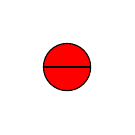
\begin{tikzpicture}[anchor=base,baseline=-3]
    \draw [fill=red] (0,0) circle (0.3);
    \draw (-0.3,0) -- (0.3,0);
    \path (-0.5,-0.5) rectangle ++(1,1); % background rectangle to unify every cell containing a symbol
  \end{tikzpicture} &
  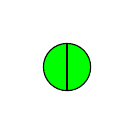
\begin{tikzpicture}[anchor=base,baseline=-3]
    \draw [fill=green] (0,0) circle (0.3);
    \draw (0,-0.3) -- (0,0.3);
    \path (-0.5,-0.5) rectangle ++(1,1); % background rectangle to unify every cell containing a symbol
  \end{tikzpicture}
  \\
    \IfLanguage{english}{distant signal}
    \IfLanguage{ngerman}{Vorsignal}
  &
  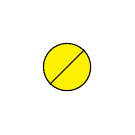
\begin{tikzpicture}[anchor=base,baseline=-3]
    \draw [fill=yellow] (0,0) circle (0.3);
    \draw (-0.22,-0.22) -- ++(0.44,0.44);
    \path (-0.5,-0.5) rectangle ++(1,1); % background rectangle to unify every cell containing a symbol
  \end{tikzpicture} &
  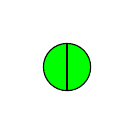
\begin{tikzpicture}[anchor=base,baseline=-3]
    \draw [fill=green] (0,0) circle (0.3);
    \draw (0,-0.3) -- (0,0.3);
    \path (-0.5,-0.5) rectangle ++(1,1); % background rectangle to unify every cell containing a symbol
  \end{tikzpicture} \\
  \bottomrule
\end{tabular}
